\label{chapter1}

In recent years, the field of soft robotics has received a substantial increase of interest. Soft robots reshape the idea of using robots for industrial processes. Currently, rigid robots dominate the field of industrial automation, as they excel in accuracy, repeatability and load capacity. However, these robots tend to be unsafe to operate in human-centred environments. Classic robots are made from rigid material and accelerate to high velocities, that could create an unsafe environment for human operators. Additionally, these robots have limited degrees of freedom, making it harder to avoid obstacles. To evade the risk of potential harm, these robots are made from flexible material: Hence the name ``soft robots''. Furthermore, their inherently dexterous structure allows soft robots to move around obstacles. This makes soft robots robust in constantly changing environments. The foundation of soft robotic design is often found in nature and includes inspiration for material choice, locomotion, and morphology. A few examples of bio-inspired soft robots include emulated trunks \cite{hannan2003kinematics} inspired by the proboscis of an elephant, robots based on the arm of octopus \cite{wang2013visual}, and robots that replicate the movement of fish \cite{marchese2014}. Figure \ref{fig1:softexample} shows a few experimental soft robots. 


\begin{figure}[H]       
    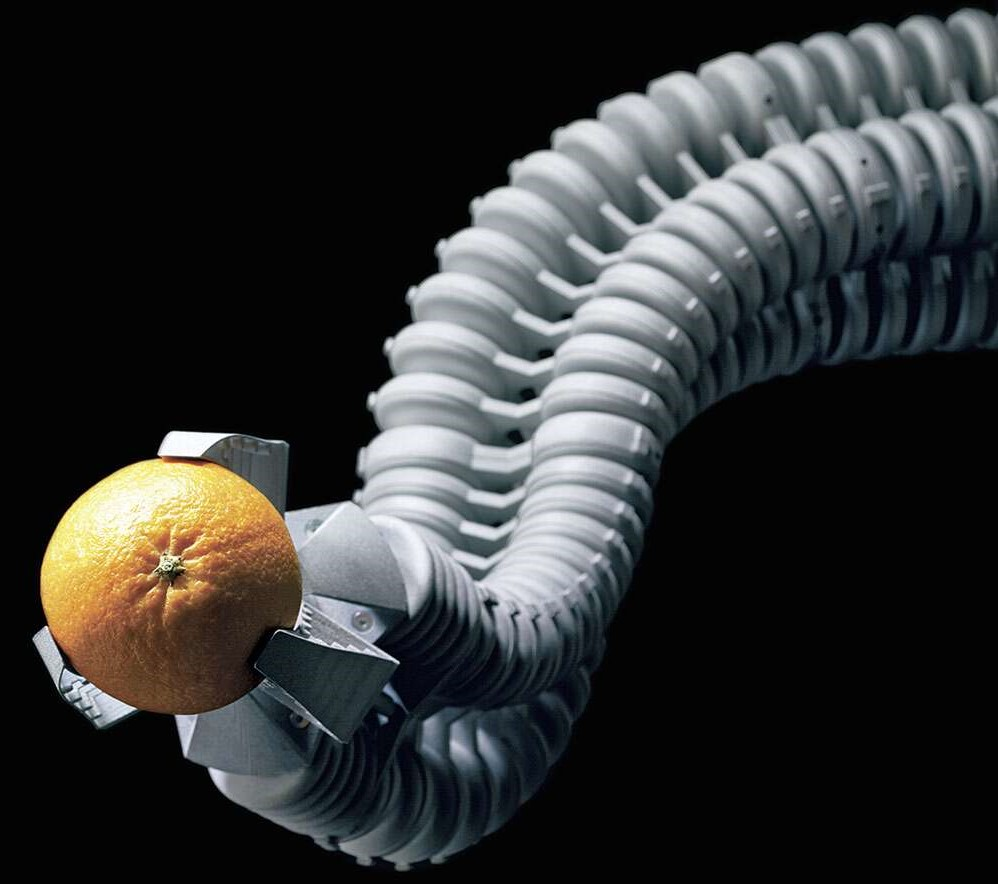
\includegraphics[width = 0.3\textwidth]{Figures/Introduction/bhasinasappel.jpg}   
    \hspace{0px}
    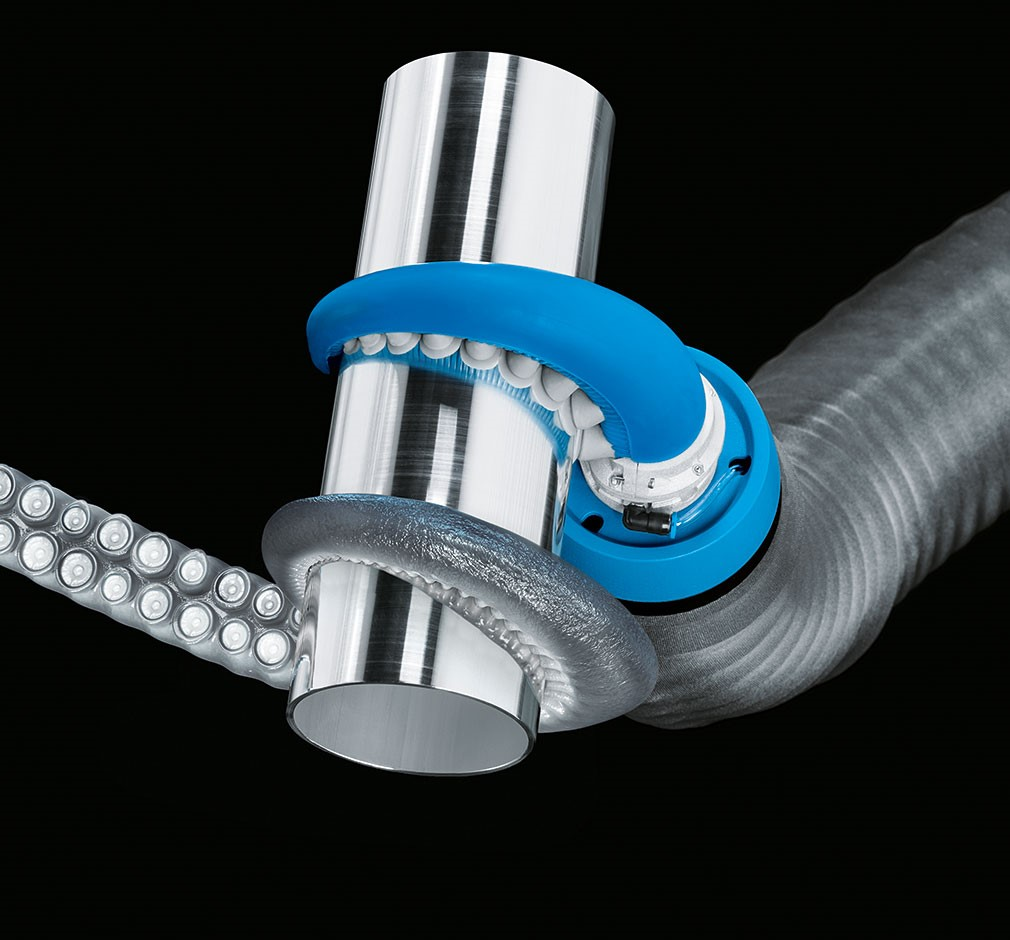
\includegraphics[width = 0.3\textwidth]{Figures/Introduction/tentaclegripper.jpg}
    \hspace{0px}
    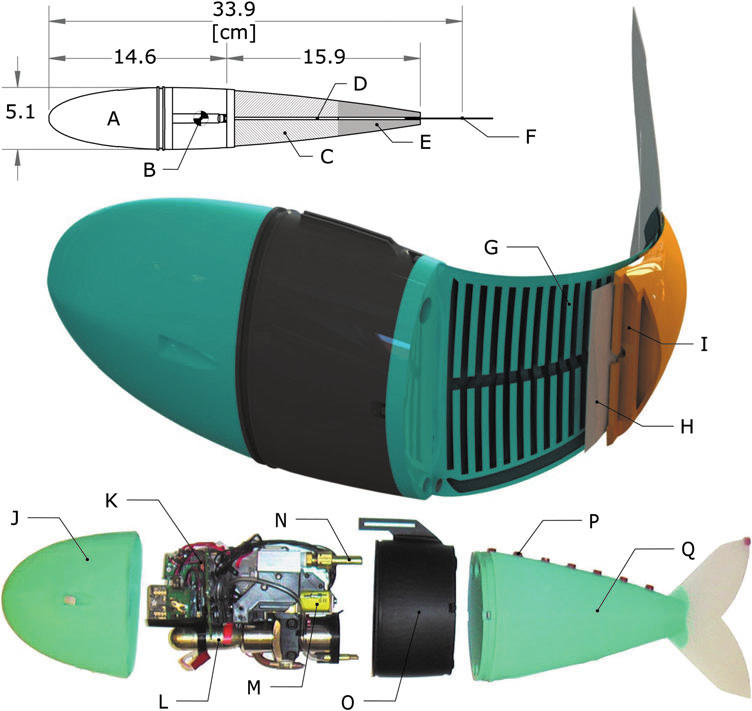
\includegraphics[width = 0.3\textwidth]{Figures/Introduction/fish.jpg}
    \caption{From left to right. Bionic Handling Assistant inspired by the trunk of an elephant \cite{BHA}. Octopus-inspired robot able to move and manipulate a wide range of objects \cite{octopus}.Bio-inspired soft robot replicating movement of a fish \cite{marchese2014}.}
    \label{fig1:softexample}
\end{figure}

There are some major differences between soft robots and the common rigid robots. First, a classification between both can be made on the basis of the compliance of their underlying materials \cite{Bionics2008}. Generally, classic robots are made of rigid metal beams, whereas soft robots are made from soft polymer materials. The building materials of the robot largely determine the kinematic redundancy of the robot. Since soft robots are composed of materials with an extremely low Young's modulus, they are able to undergo large (and possibly non-linear) deformation during normal operation. As a result of this compliance, gravity and payload cause a distributed deformation throughout the entire system . This gives the robot theoretically an infinite amount of degrees of freedom. This makes controlling these robots more challenging when compared to traditional robots, as the latter has a fixed amount of degrees of freedom.

Robot actuation is another major difference between the two robot types.
Whereas traditional robots are generally electro-mechanically actuated, soft robots can be actuated with a wide range of actuation methods, which includes pneumatics, hydraulics, thermal and even chemical \cite{BHA}, \cite{marchese2014},\cite{kang2019programmable}, \cite{shepherd2013using}. Rigid robots are often linked by rotatory or prismatic joints, where its design allows to include the actuator inside the robot. Soft robot actuators are often located externally, as their design simply does not allow to include them. Most soft robots are actuated pneumatically or by using variable length tendons \cite{Rus2015}. A well-known example of a pneumatically actuated soft robot is is the Bionic Handling assistant by Festo, as shown in Figure (\ref{fig1:softexample}). This type of soft robots have inflatable channels that cause a desired deformation when applying pressure. An example of a tendon driven is robot is the elephant trunk's robot \cite{cieslak1999elephant}. This manipulator consists of eight elastic segments linked together by coil springs. Each segment is controlled by two pairs of strings. Servo or linear actuators are used to wind and unwind the strings, with that controlling the movement of the robot. Both actuation methods introduce additional dynamics that largely affect performance of the entire control system. 

Lastly, most soft robots do not allow to use conventional sensing mechanisms. For hard robots their joint design allows to incorporate encoders to measure rotation and other sensory devices. Since the forward kinematics, given rigid joints and links, can be computed through trigonometry, position sensing is relatively easy. For soft robots, the compliant and lightweight nature often prevents the integration of conventional sensors, such as encoders, strain gauges and inertial measurement units (IMU's) \cite{Rus2015}, \cite{Lee2017}. Alternative sensory techniques are often needed. These methods include for instance optical sensors and stretch sensors based on macrobend fibres \cite{Sareh2015}.


Previous section discussed the contrast between rigid robots and soft robots. It showed that soft robots distinct themselves from traditional robots on three fronts. Their inherent soft body leads to a theoretical infinite degree system. The actuation of soft robots introduces additional dynamics caused by the actuators. Furthermore, conventional sensory mechanism can often not be applied to soft robots, and therefore demand more complex sensory devices. These factors all effect the way soft robots can be controlled. Recent literature often tries to convey readily available control theories and apply those to soft robotics.

The work of Thuruthel et al. (2018) \cite{george2018control} presents an overview of recent findings in soft robotic control for pneumatic actuated and tendon-driven soft robots. In this work, three control approaches are distinguished, namely model-free, hybrid and model-based control. A model-free control strategy does not use kinematic or dynamical description in its control approach. Instead, it exploits learning-based algorithms to dynamically control the robotic system. Hybrid controllers combine learning or empirical elements with a model-based approach. The model-based controllers rely on a analytical description of robotic system. Furthermore, for each control approach, a sub-division between kinematic and dynamical control is made. Here, kinematic control is defined as a zero order input-output relation. A change in input is directly observed in output, therefore this approach is lower-level compared to dynamical control. For the latter, the configuration space and/or task space variables' velocities are used in the control algorithm. 


Research conducted on the Bionic Handling Assistant (BHA), as shown in Figure \ref{fig1:softexample}, demonstrates that multiple control methods can be applied to the same robot. A model-free control approach was implemented in \cite{rolf2013efficient}. The inverse kinematics of the robot were obtained through machine learning, instead of model-derivation. Later work shows the implementation of a hybrid controller \cite{reinhart2017hybrid}. In this approach, an inverse kinematic model was used together with a learning model. Previous to this hybrid controller, a model-based controller was proposed by \cite{mahl2014bhakin}. However, this model-based controller only used a kinematic description of the soft robot. This research was followed up by \cite{falkenhahn2016dynamic}, which developed a dynamic controller. In this work the system is controlled with a nonlinear length controller based on feedback linearization. This controller was further supported by linear PD and feedforward control. 

In \cite{wang2013visual} visual servo control is used to control a cable-driven soft robotic manipulator. The manipulator, inspired by an octopus' tentacle, is shaped like a cone. On the outer surface of the soft robot four cables are uniformly distributed. These cables are on one end connected to the tip of the manipulator and on the other side connected to pulleys. By winding and unwinding the cables on the pulleys, the end-effector can be positioned in the task space. A kinematic-based visual servo controller is designed, based on linear PD feedback control with gravity compensation. Position sensing is done by a camera mounted at the tip of the robot, and a fixed feature point. Based on this visual information, a jacobian matrix is estimated, which is used in the kinematic controller.

In \cite{zhang2017visual} also visual servo control was implemented to control a tendon-driven soft robotic manipulator. Again, kinematic control is used for a reference tracking problem. Contrary to the previous research, where a jacobian matrix is estimated, here the jacobian is calculated by running a real-time FEM model parallel. A control architecture is set-up in which the reference input is ran through the FEM model, which outputs a jacobian and expected end-effector position. The jacobian is used in the controller to control the actual manipulator. The FEM model's expected end-effector position and actual end-effector position are used in a second controller to enhance jacobian estimation in the FEM model.

A model-based controller that uses a dynamical model in its control loop is presented in \cite{della2020model}. The robots infinite dimensionality is resolved by regarding the robot being composed of six individual actuatable segments. A Piecewise Constant Curvature (PCC) approach was used to describe the kinematics of the robotic actuator. For each segment Denavit-Hartenberg (DH) is used to describe the rigid robot equivalent, which is then used to derive a dynamic model. The proposed controller essentially is a computed torque controller with an additional PD controller. 

In aforementioned work, \cite{della2020model}, the infinite dimensionality of the soft robot is solved by assuming the robot consists of a fixed amount of segments. In this way the infinite dimensionality of the system can be approximated by fixed amount of degrees of freedom. This makes controller design easier. Of course, the reduction of degrees of freedom is at the cost of model accuracy. 



\section*{Thesis outline and contribution}

% add work of Has here.

The fundamentals of this research are provided in \cite{Caasenbrood2020}, which developed a frame work to model the soft robot dynamics. This model can be valuable for soft robotic control. Therefore the research question that we try to answer is:

\textit{Can we develop a model-based control strategy for a pneumatically actuated, planar soft robot to perform a reference tracking problem?}

To provide an answer to this research question we study the robot as depicted in Figure \ref{fig1:actuator}. This soft actuator has a theoretical infinite amount of degrees of freedom, as it is composed of flexible polymer. Furthermore it is pneumatically actuated, inducing additional dynamics into the control system, and a major limiting factor on achievable bandwidth. The sensing is done with inertial measurement unit (IMU) and an optical vision sensor. 

\begin{figure}[H]
    \centering
    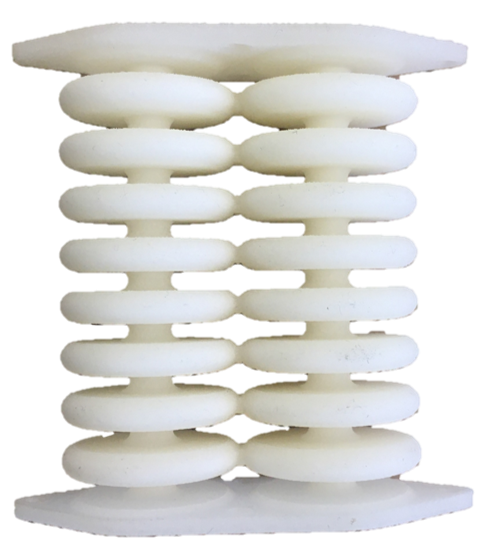
\includegraphics[width = 
   0.38\textwidth]{Figures/Chapter1/actuator.png}
    \caption{Planar soft robot manufactured from polymer}
    \label{fig1:actuator}
\end{figure}

This thesis has the following structure. In Chapter \ref{chap2} a forward kinematic description of the actuator is derived. This allows to study the robot's configuration in 2D-space. Furthermore, it allows us to study the velocity of the actuator as a function of kinematic configuration. The latter allows us to derive a dynamic model of the actuator. Once this model is derived, a parameter study is performed in Chapter \ref{chap3}. Here finite element analysis is used to capture the non-linear stiffness of the soft actuator. In Chapter \ref{chap4} a model-based controller 
is proposed. This controller will be tested in simulation, using the dynamic model as derived in Chapter \ref{chap2}. In Chapter \ref{chap5} the derived controller is experimentally verified. 

Recapitulating, this thesis includes the following:


\begin{itemize}
    \item Development of a non-linear dynamic model
    \item Determination of non-linear actuator stiffness
    \item Completing experimental set-up for the planar soft robot 
    \item Development of a model-based control law
    \item Experimental implementation of the controller
\end{itemize}

\begin{figure}[H]
    \centering
    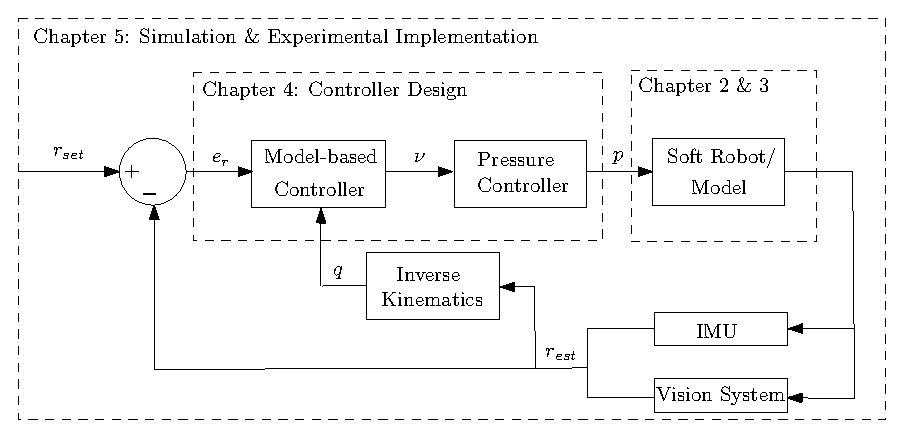
\includegraphics[width = \textwidth]{Figures/Chapter1/controlschemeComplete.eps}
    \caption{Caption}
    \label{fig:my_label}
\end{figure}




%A kinematic description of the actuator is necessary to describe the position in three-dimensional space. A widely adopted method for describing the configuration of soft robots is piece-wise constant curvature (PCC) modelling \cite{ccapproach}. Previous research used this model to describe forward kinematics of soft actuators are \cite{mahl2014bhakin}, \cite{berkers},\cite{Falkenhahn2015}, \cite{ccapproach}, \cite{runge2017framework}. A schematic drawing of the constant curvature modelling approach is shown in Figure \ref{fig2:ccapproach}. Although we will not be using this exact methodology, it is important to understand the basics. The constant curvature describes the position of the actuator by three coordinates. Parameter $l$ is the curved length of the actuator measured from the fixed bottom to the tip. Coordinate $\kappa$ expresses the curvature of the actuator. It is assumed that the deformed actuator describes a perfect arc, hence radius $r$ is equal to $\frac{l}{k}$. This allows to write the orientation of the actuator's tip as $\theta = l\kappa$. Lastly, parameter $\phi$ describes the rotation of the actuator with respect to the ground. A single constant curvature is not able to describe complex actuator configurations. To this end, multiple of these curves are stacked onto each other, thereby discretizing the actuator. This allows to describe more complex configurations. This methodology is used in for instance \cite{Falkenhahn2015}.

%The PCC approach has some limitations, due to its piece-wise character the actuator configuration is not described by a single continuous function. This makes it harder to find analytical expressions for for instance derivatives. Additionally, this PCC approach only allows to assign material properties to particular points. This makes dynamical models generally less accurate. One method to overcome this problem is using partial differential equations (PDE's) to describe actuator configurations. These PDE's are more suitable for deriving continuum dynamic models. 


\begin{figure}[H]
\centering
\begin{minipage}{.5\textwidth}
  \centering
  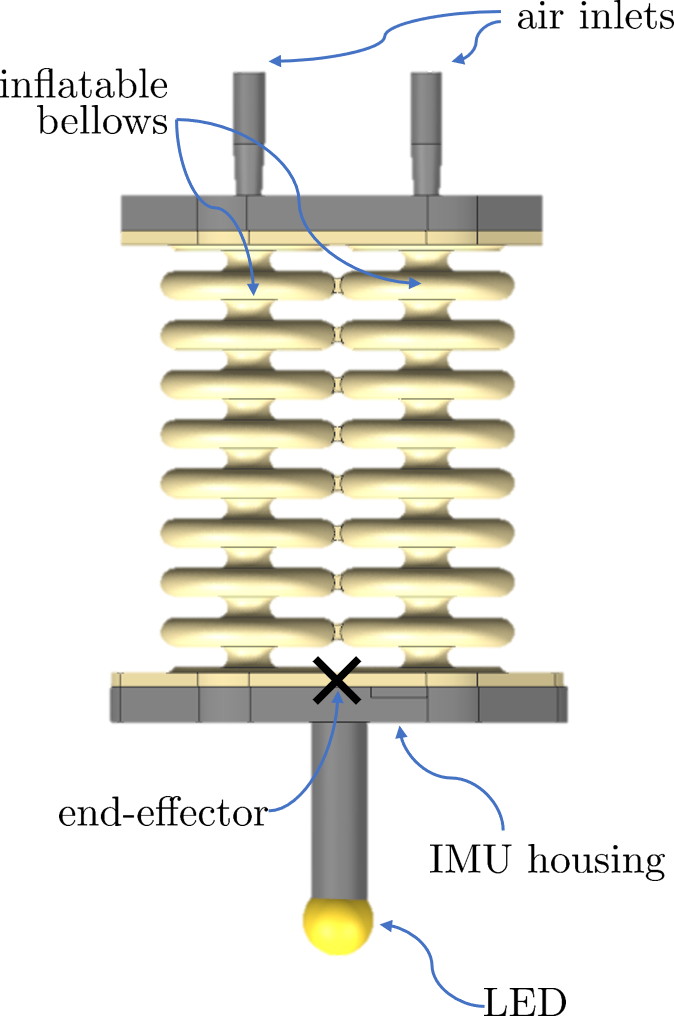
\includegraphics[width = 0.8\linewidth]{Figures/Chapter1/completesetup2.png}
  \caption{Computer rendered image of the soft robot set-up }
  \label{fig:test1}
\end{minipage}%
\begin{minipage}{.5\textwidth}
  \centering
  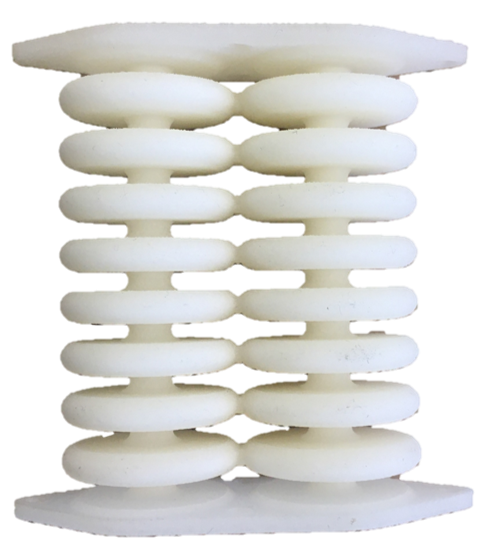
\includegraphics[width =0.8\linewidth]{Figures/Chapter1/actuator.png}
  \vspace{50pt}
  \caption{Image of the actual soft robot}
  \label{fig:test2}
\end{minipage}
\end{figure}
